%% packages
\documentclass{article}
\usepackage[a4paper, left=2.0cm, right=2.0cm, top=3.5cm]{geometry}
\usepackage[ngerman]{babel}
\usepackage{graphicx}
\usepackage{multicol}
\usepackage{amssymb}
\usepackage{titlesec}
\usepackage{wrapfig}
\usepackage{blindtext}
\usepackage{lipsum}
\usepackage{caption}
\usepackage{listings}
\usepackage{fancyhdr}
\usepackage{nopageno}
\usepackage{authblk}
\usepackage{amsmath} % tons of math stuff
\usepackage{mathtools} % e.g. alignment within matrix
%\usepackage{bm} % provides shorthand for bold in math mode
\usepackage{dsfont} % \mathds makes double stroke digits
\usepackage{esdiff} % provides \diff
%\usepackage[ISO]{diffcoeff}
\usepackage{xcolor}
\usepackage{csquotes} % e.g. provides \enquote
\usepackage[separate-uncertainty=true]{siunitx} % units
\usepackage{xcolor} % colored text
\usepackage[l3]{csvsimple}
\usepackage{subcaption}
\usepackage{physics}
\usepackage{hyperref}
\usepackage{nameref}
\hypersetup{colorlinks=true, linkcolor=black, pdfhighlight={/N}}
\usepackage{tcolorbox}
\usepackage{amsthm}
\usepackage{gensymb} % add \degree in math mode?
\usepackage{newunicodechar} % define custom unicode characters
\usepackage{booktabs}

% \sisetup{
%   scientific-notation = auto,  % Automatically use scientific notation for large/small numbers
%   output-exponent-marker = \text{e}  % (optional) for formatting the exponent symbol
% }



%\fancyhf[]{}

%% custom stuff
% own units
\DeclareSIUnit \VSS {\ensuremath{V_\mathrm{SS}}}
\DeclareSIUnit \VS {\ensuremath{V_\mathrm{S}}}
\DeclareSIUnit \Veff {\ensuremath{V_\mathrm{eff}}}
\DeclareSIUnit \Vpp {\ensuremath{V_\mathrm{pp}}}
\DeclareSIUnit \Vp {\ensuremath{V_\mathrm{p}}}
\DeclareSIUnit \VRMS {\ensuremath{V_\mathrm{RMS}}}
\DeclareSIUnit \ASS {\ensuremath{A_\mathrm{SS}}}
\DeclareSIUnit \AS {\ensuremath{A_\mathrm{S}}}
\DeclareSIUnit \Aeff {\ensuremath{A_\mathrm{eff}}}
\DeclareSIUnit \App {\ensuremath{A_\mathrm{pp}}}
\DeclareSIUnit \Ap {\ensuremath{A_\mathrm{p}}}
\DeclareSIUnit \ARMS {\ensuremath{A_\mathrm{RMS}}}

% change subsection numbering to capital letters
\newcommand{\subsectionAlph}{ \renewcommand{\thesubsection}{\arabic{section}.\Alph{subsection}} }
% change subsection numbering to lowercase letters
\newcommand{\subsectionalph}{ \renewcommand{\thesubsection}{\arabic{section}.\alph{subsection}} }
% change subsubsection numbering to lowercase letters
\newcommand{\subsubsectionalph}{ \renewcommand{\thesubsubsection}{\arabic{section}.\arabic{subsection}.\alph{subsubsection}} }
% own fig. that works with multicols
\newenvironment{Figure}
  {\par\medskip\noindent\minipage{\linewidth}}
  {\endminipage\par\medskip}
\newcommand*{\inputPath}{./plot} % prepend this command to the argument of all input commands
\graphicspath{ {./images/}{./figure/}{../plot/}{../../plot/}{../../latex/assets/}{./assets/} }
% own enviroment for definitions
\newenvironment{definition}[1]
{\begin{quote} \noindent \textbf{\textit{#1\ifx&#1& \else : \fi}} \itshape}
{\end{quote}}

\newunicodechar{°}{\degree}


% own commands
% \newcommand{\rarr}{$\to\,$} %A$\,\to\,$B
\newcommand{\defc}{black}
\newcommand{\colorT}[2][blue]{\color{#1}{#2}\color{\defc}}
\newcommand{\redq}{\color{red}(?)\color{\defc}}
\newcommand{\question}[1]{\colorT[purple]{\textbf{(#1)}}}
\newcommand{\todo}[1]{\colorT[red]{\textbf{(#1)}}}
\newcommand{\mr}{\mathrm}

%% preparation
\begin{titlepage}
    \title{Praktikum Atome, Moleküle, kondensierte Materie \\ Versuch 402: Quantelung von Energie}
    \author[1]{Carlos Pascua\thanks{s87cpasc@uni-bonn.de}}
    \author[1]{Michael Vogt\thanks{s65mvogt@uni-bonn.de}}
    \affil[1]{Uni Bonn}
    %\date{\today}
\end{titlepage}


%% document
\begin{document}

\pagenumbering{gobble}
\maketitle
\tableofcontents
\newpage
\pagenumbering{arabic}

\pagestyle{fancy}
\fancyhead[R]{\thepage}
\fancyhead[L]{\leftmark}

\section*{Einleitung}


\section{Teil l: Bestimmung des Planckschen Wirkungsquantum}
  \subsection{Theorie}

    \subsubsection{Photoeffekt}
    Der Photoeffekt beschreibt, wie Licht auf ein Metall trifft und Elektronen aus dem Metall
     herauslöst. Ein Photon besitzt eine Energie, die proportional zur Frequenz des Lichts ist, 
     und diese Energie muss ausreichen, um die Bindungsenergie des Elektrons, die sogenannte 
     Austrittsarbeit, zu überwinden. Wenn ein Photon auf ein Elektron trifft, wird ein Teil 
     seiner Energie verwendet, um das Elektron aus dem Metall zu befreien, während der Rest 
     als kinetische Energie des Elektrons übertragen wird. Die Intensität des
       Lichts beeinflusst die Anzahl der herausgelösten Elektronen, nicht aber deren Energie.
       Eine höhere Intensität bedeutet, dass mehr Photonen auf das Metall treffen und somit 
       mehr Elektronen herausgelöst werden, aber die Energie der Elektronen bleibt gleich, 
       solange die Frequenz des Lichts konstant bleibt.
       
    \subsubsection{Photozelle}
    Die Photozelle ist ein Gerät, das das Prinzip des Photoeffekts nutzt, um Lichtenergie in 
    elektrische Energie umzuwandeln. Sie besteht aus zwei Hauptkomponenten: einer Kathode, 
    die lichtempfindlich ist, und einer Anode. Wenn Licht auf die Kathode trifft, werden 
    Elektronen aus dem Material herausgelöst. Diese freigesetzten Elektronen bewegen sich 
    unter dem Einfluss eines elektrischen Feldes zur Anode. Der resultierende Strom, der durch 
    die Bewegung der Elektronen erzeugt wird, kann genutzt werden, um elektrische Energie zu 
    liefern. Die Kathode besteht aus einem Material mit geringer Austrittsarbeit, wie 
    beispielsweise Zink, das die Elektronen leicht freisetzt, wenn es beleuchtet wird. Die 
    Intensität des Lichts bestimmt dabei, wie viele Elektronen freigesetzt werden, während 
    die Frequenz des Lichts die Energie der Elektronen beeinflusst. Der erzeugte Strom ist proportional zur Lichtintensität, was 
    bedeutet, dass bei stärkerem Licht mehr Elektronen freigesetzt werden und somit ein 
    größerer Strom fließt.


    \subsubsection{Gegenfeldmethode}
    Die Gegenfeldmethode wird häufig verwendet, um die Austrittsarbeit \( W_A \) eines Materials 
    zu bestimmen. Dabei wird eine gegensätzliche elektrische Spannung in einer Photozelle erzeugt,
     die das emittierte Elektron ablenkt. Die Spannung, die benötigt wird, um den Elektronenstrom
      vollständig zu stoppen, ist eine direkte Messung der Austrittsarbeit des Materials. In 
      einer solchen Messung ist die kinetische Energie des Elektrons gleich der Arbeit, die das
       elektrische Feld leisten muss, um das Elektron vollständig zum Stillstand zu bringen.

Die Beziehung zwischen der Energie eines Photons \( h \cdot \nu \), der Austrittsarbeit \( W_A \) 
und der kinetischen Energie des Elektrons \( E_{\text{kin}} \) lässt sich durch die Gleichung 
\[
h \cdot \nu = W_A + E_{\text{kin}}
\]
beschreiben. In der Gegenfeldmethode wird \( E_{\text{kin}} \) durch die angelegte Gegenspannung
 \( U_0 \) bestimmt, wobei die kinetische Energie des Elektrons \( E_{\text{kin}} = e \cdot U_0 \)
  ist, wobei \( e \) die Elementarladung des Elektrons ist.

Die Photozelle ist ein praktisches Gerät, das auf diesem Prinzip beruht. Sie besteht aus einer 
Elektrode, die mit einem Lichtstrahl bestrahlt wird. Durch den Photoeffekt werden Elektronen 
freigesetzt, deren Bewegung durch eine angelegte Spannung beeinflusst wird. In Verbindung mit 
der Gegenfeldmethode kann man so die Energie der freigesetzten Elektronen messen und somit die 
Austrittsarbeit des Metalls bestimmen.

Zusammengefasst ermöglichen die Messungen des Photoeffekts in einer Photozelle unter 
Verwendung der Gegenfeldmethode eine präzise Bestimmung der Austrittsarbeit eines Materials 
sowie der Beziehung zwischen der Lichtfrequenz und der Energie der herausgelösten Elektronen.

    
\clearpage
\subsection{Aufbau und Durchführung}
\begin{figure}[h!]
  \centering
  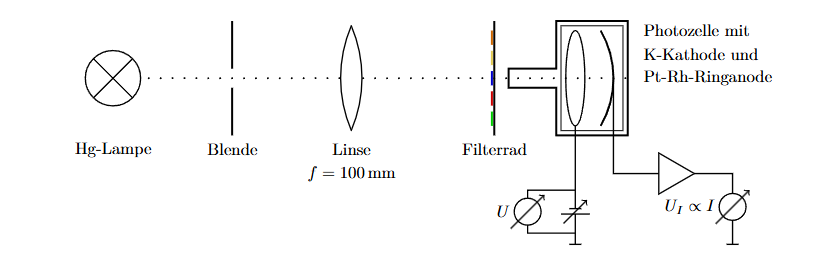
\includegraphics[width=.8\linewidth]{Aufbau_Wirkugsquantum}
  \caption{Auftragung der ersten Messung für $ \lambda =365nm$}
  \label{fig:aufbau_wirkungs}
\end{figure}

In diesem Experiment wird eine Quecksilberdampflampe als Lichtquelle verwendet. Der Lichtstrahl
 kann mit einer Blende eingegrenzt werden, um die Intensität des einfallenden Lichts zu variieren. Eine Linse wird so ausgerichtet, dass ein scharfes Bild auf der Kathode der Photozelle entsteht. Über ein Filterrad können bestimmte Linien aus dem Spektrum der Lampe isoliert werden. Direkt hinter dem Filterrad befindet sich ein Rohr, das Streulicht minimiert.

Die Photozelle selbst besteht aus einer Ringanode, die aus Platin und Rhodium gefertigt 
ist, sowie einer Kathode, die mit Kalium beschichtet ist. Beide Komponenten sind von einer 
Schutzhaube umgeben, um störendes Streulicht abzuhalten. Die Spannungsversorgung erfolgt 
durch eine regelbare Spannungsquelle im Bereich von 0 V bis 12 V. Die Spannung zwischen 
Anode und Kathode wird über einen Spannungsteiler abgegriffen, um eine präzise Justierung 
zu ermöglichen. Zur Messung der Spannung wird ein Multimeter eingesetzt. Der Strom, der 
an der Anode entsteht, wird über einen Messverstärker in eine dazu proportionale Spannung 
umgewandelt und anschließend ebenfalls mit einem Multimeter erfasst.

\subsubsection*{Justierung}
Die Justierung ist prinzipiell einfach zu verstehen. Um die optimal sicherzustellen, ist darauf zu achten, dass alle optischen 
Komponenten auf derselben Höhe positioniert und senkrecht zum Strahlengang ausgerichtet 
sind. Dabei können die Reflexionen an der Linse und am Filterrad genutzt werden, um eine 
präzise Ausrichtung zu erreichen. Die Blenden und die Linse werden so eingestellt, dass ein 
scharfes Bild der Irisblende entsteht und die Ringanode dabei nicht vom Lichtstrahl getroffen 
wird.

\subsubsection*{Durchführung}
Beide schwarzen Kabel der Photozelle (Anodenanschluss) werden mit demselben Ausgang des 
Netzgerätes verbunden. Dabei ist auf die korrekte Polung zu achten. Der Kathodenanschluss 
(weißes Kabel mit BNC-Stecker) wird mit dem entsprechenden Anschluss des Messverstärkers 
verbunden. Ein eventuell vorhandener Offset des Ausgangssignals des Messverstärkers muss 
beseitigt werden. Weiterhin wird der zweite Ausgang der regelbaren Spannung des Netzgerätes 
mit dem Masseanschluss des Messverstärkers verbunden. Die Digitalmultimeter sind so 
anzuschließen, dass sowohl der Photostrom als auch die Gegenspannung gemessen werden können.
Zunächst wird das Interferenzfilter gewählt, das das energiereichste Licht durchlässt. 
Die Gegenspannung wird so lange variiert, bis der Photostrom verschwindet. Es kann festgestellt 
werden, dass die benötigte Gegenspannung deutlich niedriger ist als die vom Netzgerät maximal 
bereitgestellte Spannung von 12 V.

Aus den vorhandenen Widerständen wird eine sinnvolle Auswahl getroffen, um den Versuchsaufbau
 um eine Spannungsteilerschaltung zu erweitern, die einen geeigneten Spannungsbereich für die
  Messungen liefert. Dieser Aufbau wird für die gesamte Messung beibehalten.

Für die Messung wird zunächst eine Wellenlänge mittels des Filterrads ausgewählt. 
Es wird die größtmögliche Gegenspannung eingestellt, und der Anodenphotostrom $I_0$ 
wird bestimmt, der aus Elektronen besteht, die aus der Anode gelöst wurden und zur 
Kathode gelangen. Anschließend wird die Gegenspannung variiert, um grob die Grenzspannung
 $U_0$ zu bestimmen, bei der der Photostrom verschwindet. Es wird die Kennlinie der 
 Photozelle aufgenommen, indem die Gegenspannung von $U = 0\,\mathrm{V}$ bis zu einer 
 Spannung variiert wird, bei der der Photostrom den Wert von $I_0$ erreicht. Dabei 
 werden Messpunkte in geeigneten Abständen aufgenommen; insbesondere ist darauf zu achten, 
 dass im quadratischen Bereich der Kennlinie genügend Messpunkte vorliegen.
Diese Messung wird für alle Wellenlängen durchgeführt ($I_0$, $U_0$, Kennlinie). 
Die Messungen der Kennlinien werden zweimal wiederholt, da die Intensität der Hg-Lampe schwankt.

Das Interferenzfilter mit der Durchlasswellenlänge $\lambda = 365\,\mathrm{nm}$ wird in den 
Strahlengang gestellt. Die erste Irisblende wird so angepasst, dass der Photostrom bei 
$U = 0\,\mathrm{V}$ deutlich größer wird. Führt eine Öffnung der Blende nicht zu einer 
Erhöhung des Photostroms, wird der Blendendurchmesser so weit verringert, bis eine deutliche 
Abnahme des Photostroms um $30\%-50\%$ beobachtet werden kann. Die Kennlinie der Photozelle 
wird für diese Wellenlänge wie zuvor beschrieben bei dieser niedrigeren Intensität aufgenommen.

\subsection{Auswertung}
Um die Energiebilanz in der Photozelle zu bestimmen, werden die Anoden- und Kathodenmaterialien 
so gewählt, dass die Austrittsarbeit \( W_A \) der Anode größer ist als die der Kathode. 
In den Abbildungen [\ref{fig:fermi}] und [\ref{fig:energie}] werden sowohl die Bindungsenergie 
der äußersten Elektronen als auch die Beziehung zwischen Kathoden- und Anodenmaterialien im 
Kurzschlusszustand dargestellt.
\begin{figure}[h!]
  \centering
  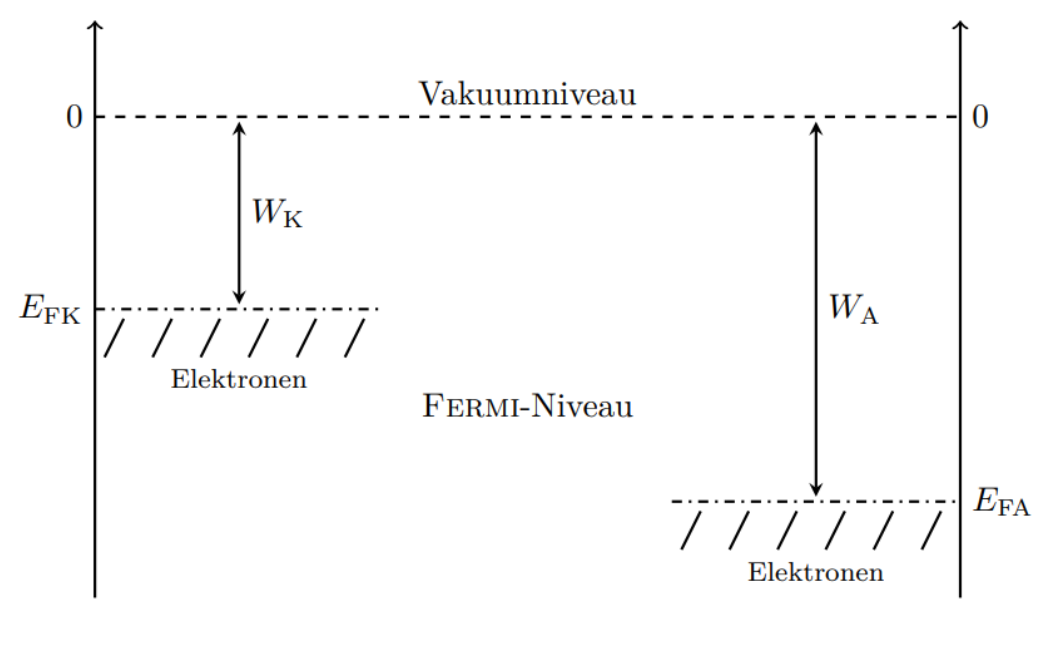
\includegraphics[width=.4\linewidth]{P402_fermi}
  \caption{Auftragung der ersten Messung für $ \lambda =365nm$}
  \label{fig:fermi}
\end{figure}
Wenn beide Materialien in einem Kurzschlusszustand verbunden werden, führen die 
Veränderungen ihrer Fermi-Niveaus zu einem Stromfluss, bis die Fermi-Niveaus wieder 
auf derselben Höhe liegen. Dies führt zur Entstehung eines Kontaktpotentials \( U_K \),
 welches sich aus der Differenz der Austrittsarbeiten der beiden Materialien bestimmen lässt.
\[
W_A = W_K + eU_K
\]
Anschließend wird eine Spannungsquelle mit einem variablen Potential
 \( -e \cdot U_G \) eingeführt, wodurch die Fermi-Niveaus um diesen Betrag verschoben werden.
Im Rahmen des Photoeffekts ergibt sich die vollständige Gleichung wie folgt:
\begin{equation}
  E = h \nu = e U_{K} + W_K + e U_G = e U_G + W_A
  \label{eq:energie}
\end{equation}
\begin{figure}[h!]
  \centering
  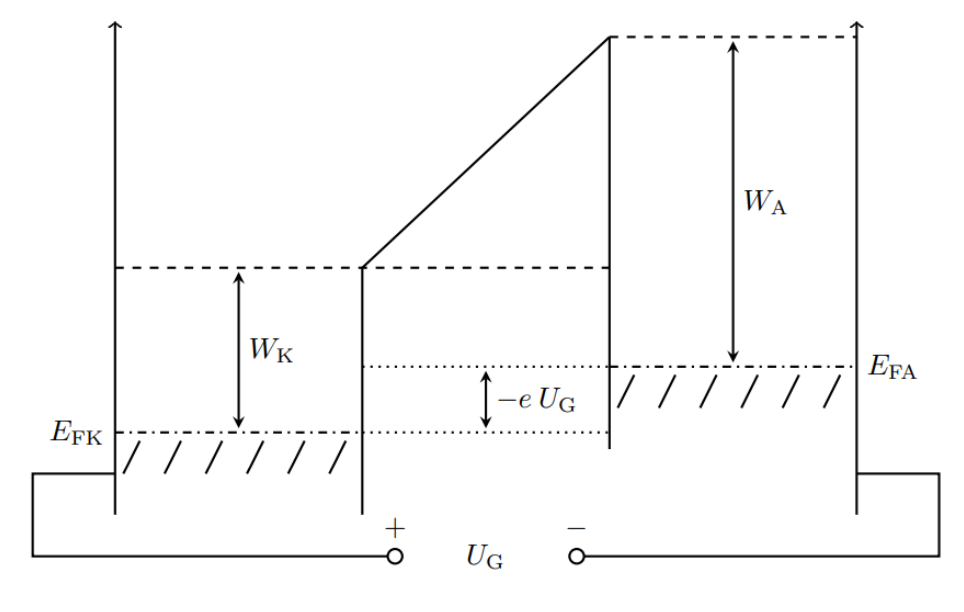
\includegraphics[width=.4\linewidth]{P402_energie}
  \caption{Auftragung der ersten Messung für $ \lambda =365nm$}
  \label{fig:energie}
\end{figure}
\newpage
\subsubsection*{Bestimmung der Grenzspannung $U_0$}
Nun werden die Photospannungswerte in einer Tabelle hinzugefügt 
(siehe Beispiel [\ref{tab:messung1a_in_main}]), und der Photostrom wird mithilfe 
eines Verstärkungsfaktors umgerechnet. Um einen linearen Zusammenhang zu 
finden, wird der Quadratwurzeloperator angewendet, ebenso wie der Wert des 
Photostroms bei maximaler Gegenspannung. Der Fehler wird unter Verwendung der bekannten
 Gaußschen Fehlerfortpflanzung bestimmt.

\begin{table*}[h!]
  \centering
  \begin{tabular}{|c|c|}
      \hline
      $U_G$ [mV] & $I$ [pA] \\
      \hline
      0.5   & 97.5 \\
      219.9 & 66.1 \\
      425   & 49.3 \\
      599   & 36.8 \\
      798   & 24.0 \\
      1009  & 16.0 \\
      1201  & 7.5  \\
      1414  & 3.0  \\
      1606  & 0.7  \\
      1805  & 0.4  \\
      2092  & 0.3  \\
      2394  & 0.2  \\
      2781  & 0.1  \\
      \hline
  \end{tabular}
  \caption{erste Messung bei 365 nm}
  \label{tab:messung1a_in_main}
\end{table*}
Der Fehler der gemessen Photostrom wird von uns gewählt und wegen große Schwankungen an der Messgeräte 
wird zu $10\%$ der gemessen Photostrom $I$.
Die Werte werden aufgetragen und eine lineare Anpassungsgerade der Form 
$f(x) = m \cdot x + b $ gelegt. Der ganze Vorgang lässt sich in einer Abbildung [\ref*{fig:wellenlaenge_365nm_a_in_main}]
darstellen. 
\begin{figure}[h!]
  \centering
  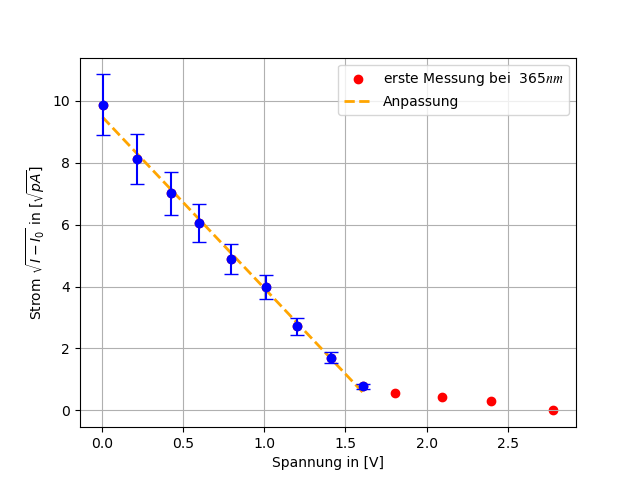
\includegraphics[width=.5\linewidth]{402_365nm_a}
  \caption{Auftragung der ersten Messung für $ \lambda =365nm$}
  \label{fig:wellenlaenge_365nm_a_in_main}
\end{figure}
\newpage

Zunächst werden alle Parameter der Anpassungsgeraden für alle Wellenlänge in der Tabelle [\ref*{tab:wellenlaengen_trennstrich_m_b_U_gemittelt}]
hinzugebracht. Diese sind wichtig, denn die Grenzspannung $U_0$ sich damit herausfinden lässt. 
\\Es gilt also: 
\begin{equation}
  U_0 = \abs*{\frac{m}{b}}
\end{equation}
\\ Der Fehler $\Delta U_0$ wird wieder mit dem Gaußschen Fehlerfortpflanzung ausgerechnet. 
$\overline{U_0}$ ist einer gemittelte Parameter aus den 2 Messungen in der gleichen Wellenlänge.
\begin{table}[h!]
  \centering
  \begin{tabular}{|c|c|c|c|c|}
  \hline
  $\lambda$ in [nm] & $m \pm \Delta m$ in [$\frac{\sqrt{pA}}{V}$] & $b \pm \Delta b$ in [$\sqrt{pA}$] & $U_0 \pm \Delta U_0$ in [V] &  $\overline{U_0}$ in [V] \\ \hline
  365 & -5.55 $\pm$ 0.35 & 9.50 $\pm$ 0.37 & 1.71 $\pm$ 0.13 & 1.72 $\pm$ 0.13 \\ \hline
  - & -5.74 $\pm$ 0.36 & 9.99 $\pm$ 0.37 & 1.74 $\pm$ 0.13 & - \\ \hline
  405 & 6.34 $\pm$ 0.36 & 8.38 $\pm$ 0.41 & 1.32 $\pm$ 0.10 & 1.32 $\pm$ 0.10 \\ \hline
  - & -6.33 $\pm$ 0.36 & 8.36 $\pm$ 0.39 & 1.32 $\pm$ 0.10 & - \\ \hline
  435 & -13.52 $\pm$ 0.51 & 15.96 $\pm$ 0.58 & 1.18 $\pm$ 0.06 & 1.16 $\pm$ 0.06 \\ \hline
  - & -13.94 $\pm$ 0.54 & 15.70 $\pm$ 0.62 & 1.13 $\pm$ 0.06 & - \\ \hline
  546 & -28.29 $\pm$ 1.6 & 17.18 $\pm$ 0.97 & 0.61 $\pm$ 0.05 & 0.62 $\pm$ 0.05 \\ \hline
  - & -26.67 $\pm$ 1.5 & 16.73 $\pm$ 0.91 & 0.63 $\pm$ 0.05 & - \\ \hline
  578 & -24.56 $\pm$ 1.6 & 11.32 $\pm$ 0.84 & 0.46 $\pm$ 0.05 & 0.46 $\pm$ 0.05 \\ \hline
  - & -23.79 $\pm$ 2.0 & 10.63 $\pm$ 0.76 & 0.45 $\pm$ 0.05 & - \\ \hline
  \end{tabular}
  \caption{Wellenlängen mit den Parameter für $m$, $b$, $U_0$ und  $\overline{U_0}$}
  \label{tab:wellenlaengen_trennstrich_m_b_U_gemittelt}
\end{table}
\clearpage
\subsubsection*{Bestimmung der Wirkugsquantum $h$ und Austrittsarbeit $W_A$}
Nun wollen wir mithilfe der zuvor bestimmten Grenzspannung \( U_0 \) das Plancksche Wirkungsquantum \( h \) 
sowie die Austrittsarbeit \( W_A \) bestimmen. Dazu wird der lineare Zusammenhang zwischen der Frequenz \( \nu \) und der 
Grenzspannung \( U_0 \) genutzt (siehe Gleichung~\ref*{eq:energie}). Es gilt:

\begin{equation}
  U_0 = \underbrace{\frac{h}{e}}_{\text{Steigung } u} \cdot \nu - \underbrace{\frac{W_A}{e}}_{\text{Achsenabschnitt } c}
\end{equation}
trägt man die Werte aus der Tabelle [\ref*{tab:wellenlaengen_trennstrich_m_b_U_gemittelt}] für die Grenzspannung und Frequenz auf 
und erhält man die folgende Abbildung.\\
\begin{figure}[h!]
  \centering
  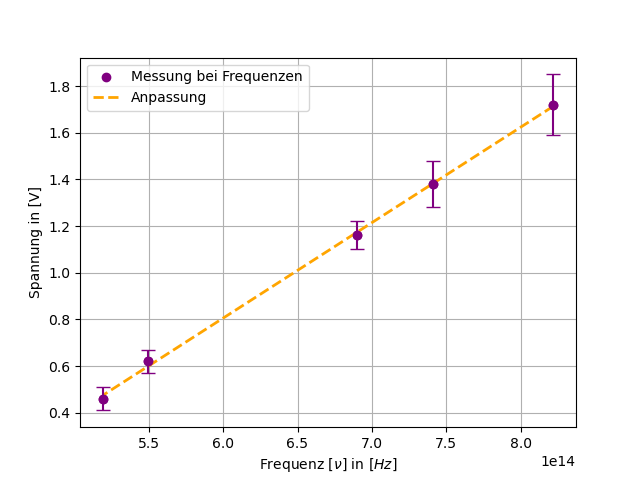
\includegraphics[width=.5\linewidth]{402_wirkung}
  \caption{Auftragung der Grenzspannung $U_0$ gegen der Frequenz $\mu$}
  \label{fig:wirkungs}
\end{figure}
\\ Zunächst lässt sich aus den Parameter der Steigung $u$ und Achsenabschnitt $c$ das
 Wirkugsquantum $h$ bestimmen. Aus Abbildung finden sich die folgenden Parameter: 
\begin{align}
  u &= (4.09 \pm 0.30) \times 10^{-15} \, \mathrm{Vs}\\
  c &= -1.65 \pm 0.18
\end{align}
Jetzt mit dem Literaturwert der Elementarladung  
\[
e = 1{,}602\,176\,634 \cdot 10^{-19}\,\mathrm{C},
\]  
entnommen aus Wikipedia \cite{elementarladung}. Für den Fehler gilt:  
\[
\Delta h = e \cdot \Delta u
\]
und  
\[
W_A = e \cdot \Delta c.
\]
Daraus ergeben sich die experimentellen Werte:


\begin{align}
  h &= (6.55 \pm 0.48) \times 10^{-34} \, \mathrm{Js}\\
  W_A &=(-2.64 \pm 0.29) \times 10^{-19} \, \mathrm{J}.
\end{align}
Der experimentelle Wert ergibt Sinn und ist innerhalb der Fehlerbalken des 
 Literaturwertes der Wirkugsquantum 
 ${\displaystyle h_{theo}=6{,}626\,070\,15\cdot 10^{-34}\;\mathrm {Js} }$. \cite{planck-h}

\clearpage
\subsubsection*{Einfluss der unterschiedlichen Intensitäten bei $\lambda = 365nm$}
Durch die Änderung des Durchmessers der Irisblende konnte der Zusammenhang zwischen
 der Lichtintensität und dem Photostrom beobachtet werden. Historisch wurde angenommen,
  dass die Energie der Elektronen von der Intensität des Lichts abhängen würde.\\
Diese Annahme wurde jedoch durch experimentelle Untersuchungen widerlegt.
 Es wurde beobachtet, dass eine höhere Lichtintensität zu einem stärkeren Photostrom führt,
  während bei geringerer Intensität ein schwächerer Photostrom resultiert.\\
Diese Beobachtung lässt sich quantenmechanisch erklären: Bei höherer Lichtintensität 
treffen mehr Photonen auf das Material, wodurch mehr Elektronen aus der Metalloberfläche 
herausgelöst werden.




\subsection{Diskussion}
\clearpage
\section{Balmer-Serie}
Es soll anhand einer Balmer-Lampe die Balmer-Serie von Spektrallinien des Wasserstoffs beobachtet und aus den Ergebnissen
die Rydberg-Konstante sowie das Plank'sche Wirkungsquantum bestimmt werden. Außerdem wird die Isotopieaufspaltung zwischen Wasserstoff und Deuterium quantifiziert.

Als Balmer-Serie bezeichnet man eine bestimmte Reihe von Spektrallinien des Wasserstoffatoms, die besonders gut mit dem bloßen Auge zu sehen sind
und 1885 von Johann Jakob Balmer untersucht wurden \cite[S. 99]{demtröder3}. Sie werden i.d.R. mit griechischen Buchstaben bezeichnet (siehe Tab. \ref{tab:balmer-literatur})
Das Vorhandensein diskreter Linien ist ein bedeutendes Beispiel der Quantelung von Energie.
Balmer fand empirisch eine Gleichung für die inverse Wellenlänge, welche einem Spezialfall der Rydberg-Formel
\begin{equation}
  \frac{1}{\lambda} = R \left(\frac{1}{n^2} - \frac{1}{m^2}\right)\ \cite{demtröder3} \label{eq:rydberg-formel}
\end{equation}
mit $R$ der \textit{Rydberg-Konstante} und $n=2$ entspricht.

Dieser Zusammenhang konnte schließlich mit dem Bohrschen Atommodell erklärt werden, demzufolge Elektronen auf diskreten Bahnen um den Atomkern kreisen
und Licht einer bestimmten Wellenlänge aussenden, wenn sie von einer höheren auf eine tiefere Bahn übergehen.
Die Balmer-Serie entspricht in diesem Modell den Übergängen der Elektronen von der $m$-ten ($m>2$) Schale auf die zweite Schale.

Heute kann das Verhalten stattdessen mithilfe der Quantenmechanik beschrieben werden, welche ebenfalls diskrete Energieniveaus der Elektronen vorhersagt.
Die Rydberg-Konstante kann theoretisch berechnet werden und es gilt
\begin{equation}
  R = \frac{\mu e^4}{8c\epsilon_0^2 h^3}~\cite[S.101]{demtröder3} \label{eq:rydberg-konstante} 
\end{equation}
mit $\mu$ der reduzierten Masse von Elektron und Kern $\mu = \frac{m_e m_K}{m_e+m_K}$.
Der Wert von $R$ hängt also von der Masse des Kerns ab. Für verschiedene Isotope des Wasserstoffs sind Linien mit leicht unterschiedlichen Wellenlängen
zu erwarten, was als \textit{Isotopieaufspaltung} bezeichnet wird.

\subsection{Versuchsaufbau}
Der verwendete Aufbau ist in Abb. \ref{fig:balmer-aufbau} gezeigt.
\begin{figure}[h]
  \centering
  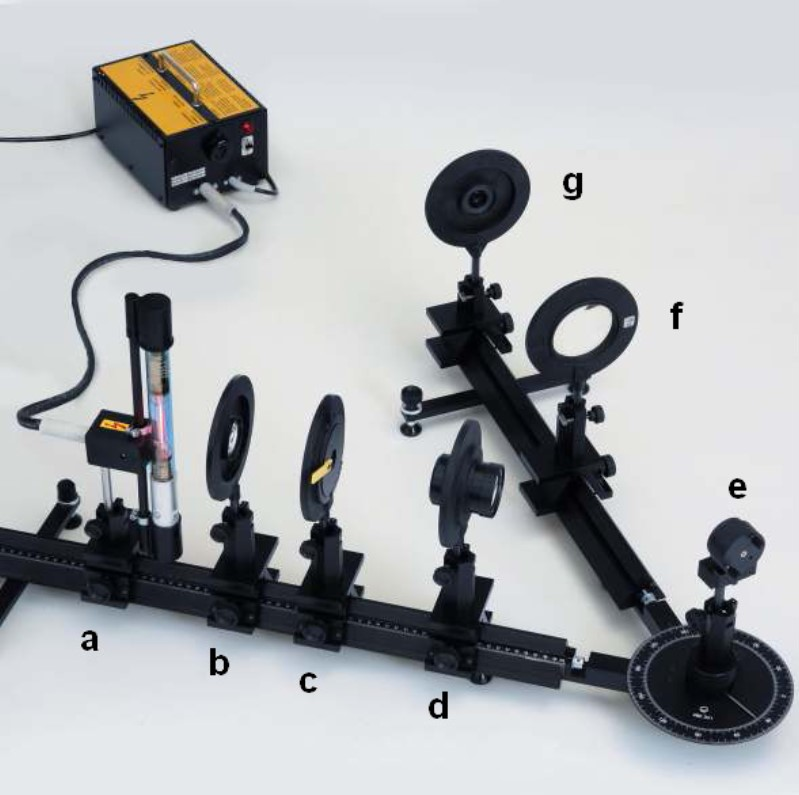
\includegraphics[width=0.5\textwidth]{balmer-aufbau}
  \caption{Aufbau zur Durchmessung der Balmer-Serie \cite{Anleitung}}
  \label{fig:balmer-aufbau}
\end{figure}
Die Linien sollen hier anhand einer Balmer-Lampe (a) beobachtet werden, welche herkömmliches sowie deuteriertes Wasser enthält.
Der Wasserdampf wird in der Lampe durch eine hohe Spannung zum Leuchten angeregt. Das Licht geht durch eine Linse (b), einen Spalt (c) 
und eine weitere Linse (d), welche als Projektionsobjektiv zur Kollimation dient, auf ein drehbar gelagertes Reflexionsgitter (e), welches hier als Interferometer dient. Das Muster kann an einer weiteren
drehbaren Schiene beobachtet werden, wo das Licht von einer weiteren Linse (f) auf das Okular (g) abgebildet wird.

Am Drehgelenk unter dem Gitter gibt es eine Winkelskala. Das Gitter wird zunächst auf \ang{0} gedreht und das Projektionsobjektiv in seinem Brennweitenabstand
(\SI{150}{\mm}, \cite{Anleitung}) hinter dem Spalt aufgestellt. Bei angeschalteter Lampe ist nun ein Bild des Spalts leicht neben dem Spalt zu sehen.
Damit das Gitter genau justiert ist, wird es in seiner Aufhängung so gedreht, dass das Bild des Spalts im Spalt selbst liegt.

Das Gitter wird gedreht, bis am Okular eine Linie sichtbar wird. Diese kann durch verschieben der Linse vor dem Okular scharf gestellt werden.
Die relevanten Winkel sind in Abb. \ref{fig:balmer-winkel} gezeigt. Wir haben für alle Messungen $\omega_B = \ang{140}$ werwendet.
Der Winkel des Gitters $\omega_G$ wird verändert, um unterschiedliche Linien zu betrachen. Für die Winkel $\alpha$ und $\beta$, welche
direkte Relevanz für die Gittergleichung haben, ergeben sich dann durch
\begin{align}
  \alpha &= \omega_G \nonumber \\
  \beta &= \ang{180} + \omega_G - \omega_B \label{eq:balmer-winkel}
\end{align}
Die Gittergleichung für konstruktive Interferenz lautet
\begin{equation}
  k\lambda = g(\sin(\alpha) + \sin(\beta)) \label{eq:gittergleichung}\ \cite{leybold-balmer}
\end{equation}
wobei hier immer die erste Ordnung mit $k=1$ beobachtet wird. $g$ ist die sogenannte Gitterkonstante,
die experimentell anhand des bekannten Spektrums von Quecksilber bestimmt werden soll.

\begin{figure}[h]
  \centering
  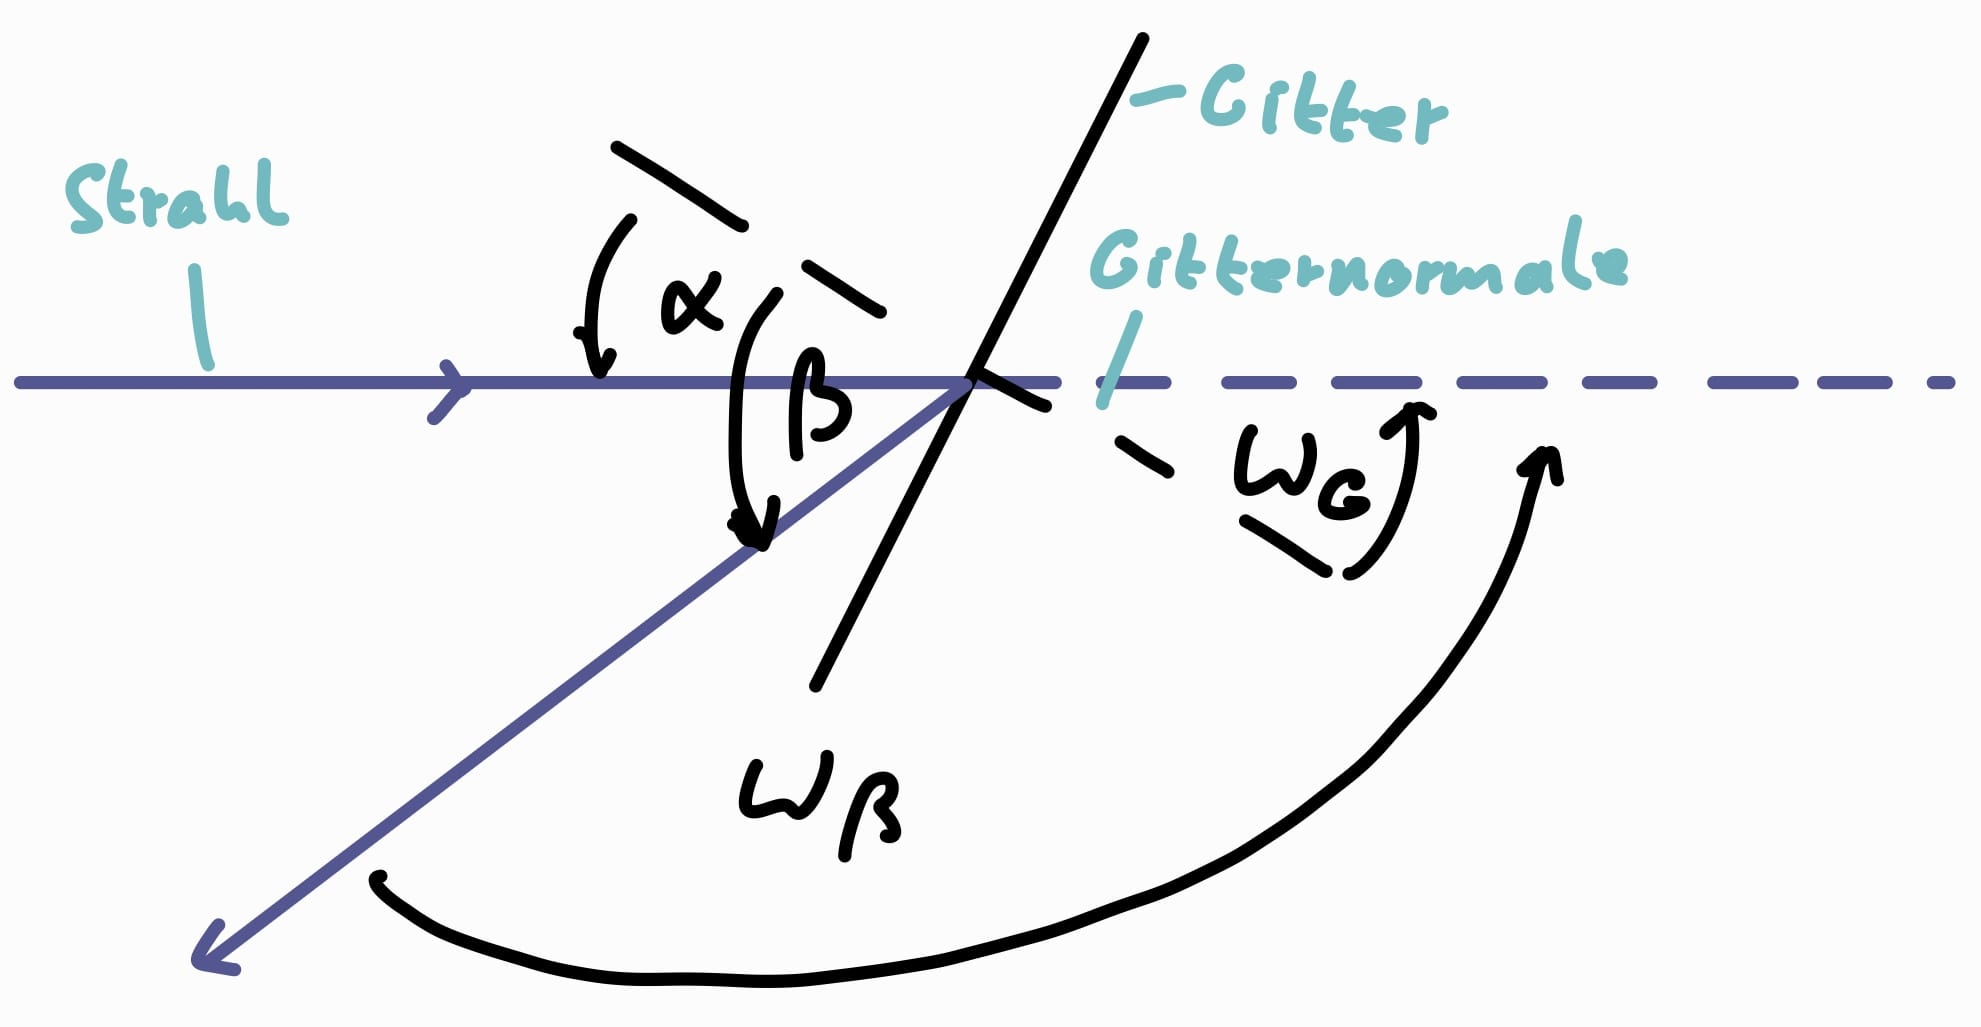
\includegraphics[width=0.5\textwidth]{balmer-winkel}
  \caption{Winkel bei der Messung der Balmer-Serie.}
  \label{fig:balmer-winkel}
\end{figure}

Das Okular hat außerdem eine Strichskala, welche dazu dient, kleine Winkelunterschiede zu messen und
hier für die Bestimmung der Isotopieaufspaltung verwendet werden kann.
% Das Zentrum der Skala liegt bei \SI{5}{\mm} und
Der Winkelunterschied zwischen zwei Linien bei $d_1$ und $d_2$ auf der Skala ergibt sich aus dem Abstand zur Abbildungslinse:
\begin{equation}
  \delta \beta = \tan^{-1}\left(\frac{\delta d \rvert}{f}\right) \tan^{-1}\left(\frac{\lvert d_2-d_1 \rvert}{f}\right) = \left\lvert \frac{d_2-d_1}{f} \right\rvert \label{eq:winkelunterschied}
\end{equation}
wobei im dritten Schritt die Kleinwinkelnäherung verwendet wurde und $f=\SI{300}{\mm}$ die Brennweite der Linse ist \cite{Anleitung}.

\subsection{Bestimmung der Gitterkonstanten}
Zunächst soll die Gitterkonstante $g$ des verwendeten Gitters bestimmt werden.
Hierzu sollen die Winkel verschiedener Hg-Linien gemessen und mit den bekannten Linien verglichen werden (Tab. \ref{tab:hg-linien}).
Zunächst wird also die Balmer-Lampe durch eine Hg-Spektrallampe ersetzt.
\begin{table}[h]
  \centering
  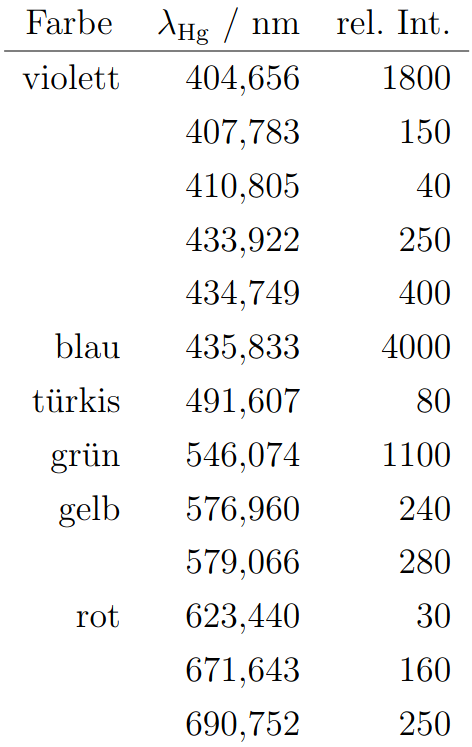
\includegraphics[width=0.2\textwidth]{hg-linien}
  \caption{Wellenlängen, Farben und Intensitäten des Hg-Spektrums. \cite{Anleitung}}
  \label{tab:hg-linien}
\end{table}

Die Winkel der beobachteten Linien zusammen mit der Farbe und der beobachteten Intensität (grobe Skala von $1$ bis $5$)
sind in Tab. \ref{tab:hg-beobachtung} gezeigt. Die Wellenlänge wurde anhand dieser Daten und Tab. \ref{tab:hg-linien} zugeordnet.
\begin{table}[h]
  \centering
  \begin{tabular}{llSSSSS}
    \toprule
    Farbe & Intensität & {$\lambda/\si{nm}$} & {$\alpha/^\circ$} & {$\beta/^\circ$} & {$g/\si{nm}$} & {$\Delta g/\si{nm}$} \\
    \midrule
    Violett & 5 & 404.66 & 11.0 & 51.0 & 418.1 & 5.3 \\
    Violett & 3 & 407.78 & 11.2 & 51.2 & 418.9 & 5.2 \\
    Violett & 1 & 410.81 & 11.6 & 51.6 & 417.2 & 5.1 \\
    Blau-Türkis & 1 & 433.92 & 13.6 & 53.6 & 417.2 & 4.8 \\
    Blau & 5 & 435.83 & 13.9 & 53.9 & 415.8 & 4.7 \\
    Türkis & 4 & 491.61 & 18.9 & 58.9 & 416.6 & 4.0 \\
    Grün & 5 & 546.07 & 24.2 & 64.2 & 416.8 & 3.4 \\
    Gelb & 4 & 576.96 & 27.5 & 67.5 & 416.4 & 3.0 \\
    Gelb & 3 & 579.07 & 27.9 & 67.9 & 415.3 & 3.0 \\
    Rot & 1 & 623.44 & 31.0 & 71.0 & 426.9 & 2.8 \\
    Rot & 1 & 671.64 & 31.6 & 71.6 & 456.0 & 2.9 \\
    Rot & 1 & 690.75 & 33.0 & 73.0 & 460.2 & 2.9 \\
    \bottomrule
  \end{tabular}
  \caption{
    Beobachtete Daten und deren Auswertung für die Linien der Hg-Spektrallampe.
    Der Fehler der Winkel wird auf \ang{0.6} geschätzt.}
  \label{tab:hg-beobachtung}
\end{table}

$\alpha$ und $\beta$ wurden anhand von \eqref{eq:balmer-winkel} berechnet und aus der Gittergleichung \eqref{eq:gittergleichung} folgt
\[
  g = \frac{\lambda}{\sin(\alpha)+\sin(\beta)}
\]
Der Fehler von g wurde mit Gauß'scher Fehlerfortpflanzung berechnet.

Für die roten Linien erhalten wir stark von den anderen Messungen abweichende Gitterkonstanten.
Womöglich haben wir hier die Wellenlängen falsch zugeordnet und sie werden für die weitere Auswertung nicht verwendet.
Um aus den restlichen Messungen einen einzelnen Wert der Gitterkonstante zu erhalten, passen wir eine Gerade
an die Gittergleichung an (Abb. \ref{fig:fit-gitterkonstante}).
\begin{figure}[h]
  \centering
  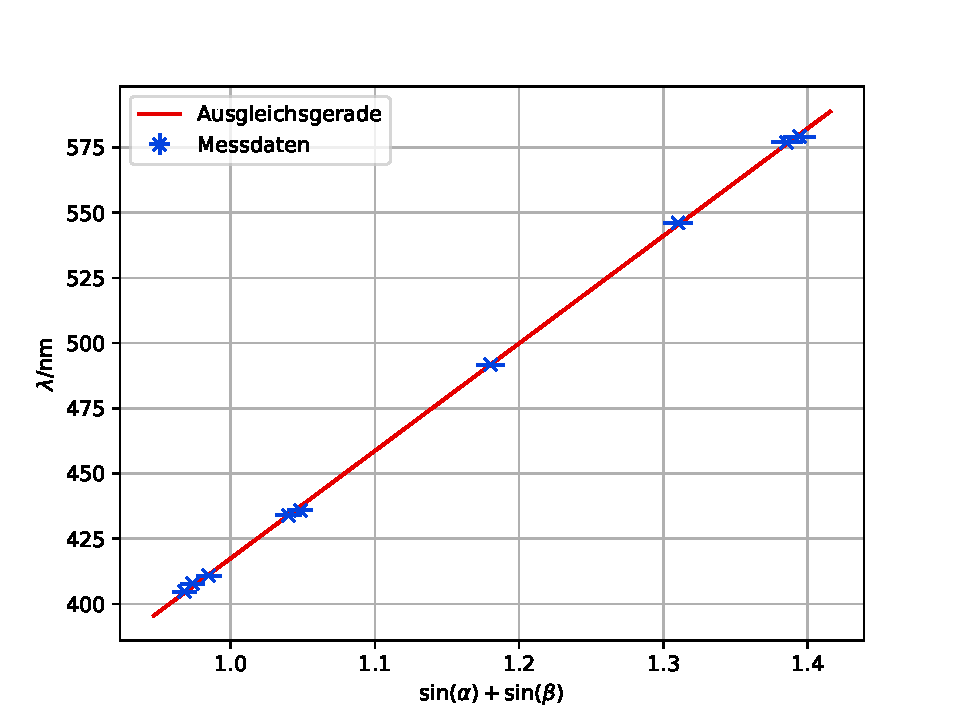
\includegraphics[width=0.5\textwidth]{fit-gitterkonstante}
  \caption{Linearer Fit zur Bestimmung der Gitterkonstante.}
  \label{fig:fit-gitterkonstante}
\end{figure}
Wir erhalten die Gleichung
\[
  \lambda = \SI{5.6\pm2.1}{\nm} + \frac{\SI{411.9\pm1.8}{\nm}}{\sin(\alpha)+\sin(\beta)}
\]
und damit
\[
  g = \SI{411.9\pm1.8}{\nm}
\]
Im Datenblatt \cite{leybold-balmer} ist angegeben,
dass das Gitter $\SI{2400}{\per\mm}$ Linien hat, was $g = \SI{416.67}{\nm}$ entspricht.
Die Abweichung von unserem Wert lässt sich dadurch erklären, dass das Gitter holographisch hergestellt wurde und
die Abstände bei solchen Verfahren nicht sehr genau sind \cite{Anleitung}, was einer der Gründe ist,
warum wir die Gitterkonstante hier selbst experimentell bestimmt haben.


\subsection{Messung der Isotopieaufspaltung}
Auf zwei verschiedene Arten soll die Isotopieaufspaltung gemessen werden. Zunächst wird das Okular verwendet und anhand
der Position entlang der Strichskala die Aufspaltung zweier Linien bestimmt. Anschließend wir das Okular durch eine
CCD-Kamera ersetzt, deren Daten am Computer exportiert werden können.

Da die Aufspaltung der Wellenlänge $\delta \lambda$ zweier Linien nur klein ist, kann ihre Abhängigkeit von der
Winkelaufspaltung $\delta\beta$ mithilfe der ersten Ableitung der Gittergleichung linear genähert werden:
\begin{equation}
  \delta\lambda = \delta\beta \cdot \diffp{\lambda}{\beta} = g\cos(\beta)\delta\beta \label{eq:balmer-aufspaltung}
\end{equation}
Die nach der Literatur erwarteten Wellenlängen und Aufspaltungen der Linien sind in Tab. \ref{tab:balmer-literatur} gezeigt.

\begin{table}[h]
  \centering
  \begin{tabular}{c||c|c|c}
    Bezeichung & $m$ & $\lambda/\si{nm}$ (bei Wasserstoff) & $\delta \lambda/\si{nm}$ \\ \hline
    H$_\alpha$ & 3 & \SI{656.28}{\nm} & \SI{0.179}{\nm} \\
    H$_\beta$  & 4 & \SI{486.13}{\nm} & \SI{0.132}{\nm} \\
    H$_\gamma$ & 5 & \SI{434.05}{\nm} & \SI{0.118}{\nm} \\
    H$_\delta$ & 6 & \SI{410.17}{\nm} & \SI{0.112}{\nm}
  \end{tabular}
  \caption{Die ersten vier Linien der Balmer-Serie und ihre Wellenlängen bei Wassserstoff (Protium) sowie die Isotopieaufspaltung. \cite{leybold-balmer}}
  \label{tab:balmer-literatur}
\end{table}


\subsubsection{Messung mit Okular}
Die beobachteten Linien und ihre Positionen entlang der Strichskala des Okulars sind in Tab. \ref{tab:balmer-messung-okular}
gezeigt. Die Mitte der Strichskala liegt bei $d = \SI{5}{\mm}$.
\begin{table}[h]
  \centering
  \csvautotabular{../data/balmer_H.csv}
  \caption{Messung der Balmer-Linien mit einem Okular, mit zugeordneter Quantenzahl $m$.
  $m=0$ bedeutet, dass wir diese Linie nicht zum Balmer-Spektrum zuordnen konnten.
  Jede Linie ist zweimal aufgeführt, für die zwei aufgespaltenen sichtbaren Peaks, die sich in ihrer Position entlang der Strichskala $d$ unterscheiden.
  $\Delta \omega_G=\ang{0.6}$, $\Delta d=\SI{0.1}{\mm}$.}
  \label{tab:balmer-messung-okular}
\end{table}

Für jede der Linien wird der Abstand $\delta d$ der Peaks berechnet und daraus
der Winkelabstand $\delta \beta$ mithilfe von \eqref{eq:winkelunterschied}.
Die Aufspaltung $\delta \lambda$ der Wellenlängen folgt dann aus \eqref{eq:balmer-aufspaltung}.
Die resultierenden Werte sind in Tab. \ref{tab:balmer-aufspaltung-okular} gezeigt.
\begin{table}
  \begin{tabular}{rSSSS}
    \toprule
    {$m$} & {$\lambda/\si{\nm}$} & {$\Delta\lambda/\si{\nm}$} & {$\delta\lambda/\si{\nm}$} & {$\Delta\delta\lambda/\si{\nm}$} \\
    \midrule
    5 & 430.7 & 5.2552 & 0.08 & 0.11 \\
    0 & 431.8 & 5.2526 & 0.08 & 0.11 \\
    4 & 478.8 & 5.1362 & 0.14 & 0.10 \\
    3 & 649.3 & 4.5762 & 0.22 & 0.04 \\
    \bottomrule
  \end{tabular}
  \caption{mit dem Okular gemessene Isotopieaufspaltung der Balmer-Linien.}
  \label{tab:balmer-aufspaltung-okular}
\end{table}

Bei allen Linien liegt der Literaturwert aus Tab. \ref{tab:balmer-literatur} im Fehlerbereich, die Fehler sind allerdings sehr groß,
da das Ablesen anhand der Strichskala im Okular schwierig war.
Um präzisere Messungen zu machen, setzen wir im Folgenden die CCD-Kamera ein.


\subsubsection{Messung mit CCD-Kamera}
wir ersetzen in dem Versuchsaufbau (Abb. \ref{fig:balmer-aufbau}) das Okular durch die CCD-Kamera,
welche über USB an einen Computer angeschlossen und dort mit einer speziellen Software ausgelesen werden kann. 
dort lässt sich die Messung in Echtzeit Beobachten und auch die Belichtungszeit justieren.
Die Software berechnet in Abhängigkeit der Pixel-Koordinate $p$ ($2048$ Pixel insgesamt) den Winkel $\gamma$ zur optischen Achse
und trägt die Intensität $I/\%$ gegen $\gamma/°$ auf.
\[
  \gamma = \arctan\left( \frac{(1024-p)\cdot \SI{0.014}{\nm}}{f} \right)\ \cite{Anleitung}
\]
Dabei ist $f=\SI{300}{\mm}$ die Brennweite der Abbildungslinse.

Um aus den CCD-Bildern die Positionen der sichtbaren Peaks zu extrahieren, wurde die an den Daten einen Fit der Form
\[
  I(\alpha) = B + G(\alpha; a_1, \mu_1, \sigma_1) + G(\alpha; a_2, \mu_2, \sigma_2)
\]
durchgeführt. Dabei wurde auf den Intensitäten ein Fehler von $\Delta I = 0.5\%$ angenommen.
Der additive Parameter $B$ ermöglicht die Berücksichtigung einer eventuell vorhanden gleichmäßigen Grundausleuchtung
und sorgt nach visueller Inspektion erfahrungsgemäß für bessere Anpassung der Gauß-Parameter an die Daten.
Es werden die verallgemeinerten Gauß-Funktionen
\[
  G(xg a, \mu, \sigma) = a \exp(\frac{(x-b)^2}{2c^2})
\]
verwendet. 
Die Plots mit Fit sind in im Anhang in Abb. \ref{fig:gauss-fit} gezeigt. Im Bild bei $\alpha=\ang{13.8}$
sind die beiden erkennbaren Maxima deutlich weiter von einander entfernt, als bei den anderen beiden Messungen.
Dies bedeutet, dass es sich hier nicht um die Aufspaltung einer Linie, sondern um zwei unterschiedlichen Linien
handelt (es handelt sich um die zwei nahe beieinander liegenden Linien, die wir auch mit dem Okular beobachten konnten, siehe Tab. \ref{tab:balmer-messung-okular}).
Daher wurde für diese Messung kein Fit durchgeführt.

die Positionen der Maxima sind in Tab. \ref{tab:gauss-parameter} gezeigt.
\begin{table}[h]
  \centering
  \begin{tabular}{SSSSSSSS}
    \toprule
    {$\alpha/°$} & {$\beta/°$} & {$\mu_1/°$} & {$\Delta\mu_1/°$} & {$\mu_2/°$} & {$\Delta\mu_2/°$} & {$\delta\beta/°$} & {$\Delta\delta\beta/°$} \\
    \midrule
    18.2 & 58.2 & -0.0307 & \num{0.00026} & \num{0.0012} & \num{0.000054} & 0.03195 & \num{0.00027} \\
    37.0 & 77.0 & -0.111 &  \num{0.000072} & \num{-0.0078} & \num{0.000020} & 0.104 & \num{0.000075} \\
    \bottomrule
  \end{tabular}
  \caption{
    gemessene Winkelpositionen der aufgespaltenen Balmer-Linien.
    $\mu_1$ und $\mu_2$ sind die aus einem $\chi^2$-Fit bestimmten Positionen der Linien und $\delta\beta$
    die Differenz der beiden. $\Delta \alpha=\Delta \beta=\ang{0.6}$.}
  \label{tab:gauss-parameter}
\end{table}

Mit den $\delta\beta$-Werten wird weitergerechnet, analog zu der Okular-Messung.
Die resultierenden Werte sind in Tab. \ref{tab:balmer-aufspaltung-ccd} gezeigt.
\begin{table}
  \centering
  \begin{tabular}{rSSSS}
    \toprule
    {$m$} & {$\lambda/\si{\nm}$} & {$\Delta\lambda/\si{\nm}$} & {$\delta\lambda/\si{\nm}$} & {$\Delta\delta\lambda/\si{\nm}$} \\
    \midrule
    4 & 478.8 & 5.1362 & 0.12 & 0.0023 \\
    3 & 649.3 & 4.5762 & 0.17 & 0.0076 \\
    \bottomrule
  \end{tabular}
  \caption{mit der CCD-Kamera gemessene Isotopieaufspaltung der Balmer-Linien.}
  \label{tab:balmer-aufspaltung-ccd}
\end{table}


\subsection{Rydberg-Konstante und Wirkungsquantum}
Aus unseren Messungen kann nach die Rydberg-Konstante bestimmt werden.
Hierzu werden die mit dem Okular gemessenen Winkel der Linien verwendet. Diese entsprechen den
Positionen der helleren Linien. Die helleren Linien sind diejenigen, die von Wasserstoff (Protium) erzeugt wurden,
denn das Mischverhältnis von Protium zu Deuterium in der Lampe ist 2:1 \cite{Anleitung}.
% Da der Fehler auf $\beta$ mit \ang{0.6} ohnehin relativ groß ist, 

nach \eqref{eq:rydberg-formel} mit $n=2$ ist $R_H$ der Betrag der Steigung von $\frac{1}{\lambda}$ in Abhängigkeit von $\frac{1}{m^2}$:
\[
  \frac{1}{\lambda} = \frac{R_H}{4} - R_H \frac{1}{m^2}
\]
Aus den Daten von Tab. \ref{tab:balmer-messung-okular} ergibt sich der $\chi^2$-Fit in Abb. \ref{fig:rydberg-fit}
\begin{figure}{h}
  \centering
  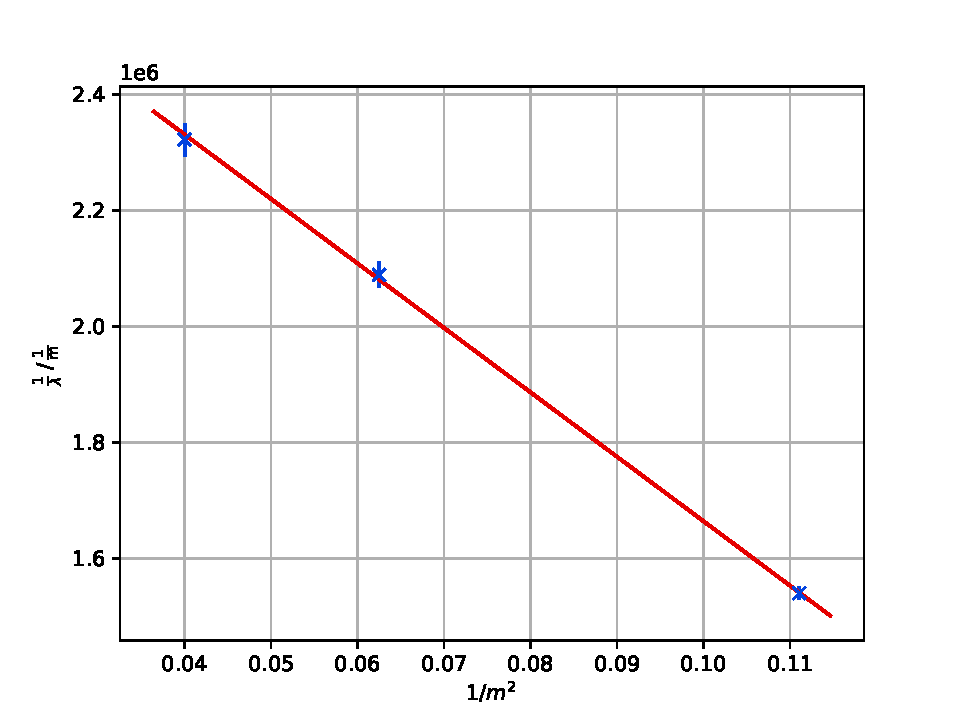
\includegraphics[width=0.5\textwidth]{rydberg_fit}
  \caption{Linearer Fit der Wellenzahl $\frac{1}{\lambda}$ zur Bestimmung der Rydberg-Konstante von Wasserstoff.}
  \label{fig:rydberg-fit}
\end{figure}
und der Zusammenhang
\[
  \frac{1}{\lambda} = \SI{0.2775\pm0.0032e7}{\per\pm} - \SI{1.111\pm0.031}{\per\m} \frac{1}{m^2}
\]
Der vierfache Achsenabschnitt und der Betrag der Steitung entsprechen beide der Rydberg-Konstante.
Der Mittelwert aus diesen beiden Werten ist
\[
  R_H = \SI{1.1104\pm0.0155e7}{\per\m}
\]
Der Literaturwert für die Rydberg-Konstante ist
\begin{equation}
  R_H \approx R_\infty = \SI{1.0974e7}{\per\m} \cite{rydberg}
\end{equation}
Hier wurde näherungsweise wurde die Rydberg-Konstante für $\mu=m_e$ verwendet, da der Unterschied deutlich
kleiner als unsere Messunsicherheit ist. Der Wert liegt innerhalb des Fehlerbereichs des experimentellen Ergebnis
und die Abweichung beträgt nur etwa $1\%$.

Aus dem experimentellen Wert für $R_\infty \approx R_H$ berechnen außerdem das Planck'sche Wirkungsquantum.
Nach \eqref{eq:rydberg-konstante} gilt
\[
  h = \sqrt[3]{\frac{m_e e^4}{8c \epsilon_0^2 R_\infty}} = \SI{6.600\pm0.037e-34}{\J\s}
\]
Der Literaturwert ist $h = \SI{6.626e-34}{\J\s}$ \cite{planck-h} und aus der Messung des Photoeffekts wurde
$h = (6.55 \pm 0.48) \times 10^{-34} \, \mathrm{Js}$ bestimmt.
Alle drei Werte stimmen innerhalb der Fehlerbereiche miteinander überein, wobei jedoch das anhand der Balmer-Linien berechnete
Wirkungsquantum eine deutlich geringere Unsicherheit hat, als der Wert vom Photoeffekt.



\clearpage
\section{Fazit}


\clearpage
\section{Anhang}
\subsection{Photoeffekt}

% Corrected Table for Messung 1a 365 nm data
\begin{table*}[h!]
  \centering
  \begin{tabular}{|c|c|}
      \hline
      $U_0$ [mV] & $I$ [pA] \\
      \hline
      0.5   & 97.5 \\
      219.9 & 66.1 \\
      425   & 49.3 \\
      599   & 36.8 \\
      798   & 24.0 \\
      1009  & 16.0 \\
      1201  & 7.5  \\
      1414  & 3.0  \\
      1606  & 0.7  \\
      1805  & 0.4  \\
      2092  & 0.3  \\
      2394  & 0.2  \\
      2781  & 0.1  \\
      \hline
  \end{tabular}
  \caption{Messung 1a bei 365 nm}
  \label{tab:messung1a}
\end{table*}

% Corrected Table for Messung 1b 365 nm data
\begin{table*}[h!]
  \centering
  \begin{tabular}{|c|c|}
      \hline
      $U_G$ [V] & $I$ [pA] \\
      \hline
      0.001  & 104.5 \\
      0.241  & 75    \\
      0.523  & 49    \\
      0.749  & 29    \\
      1.011  & 14.6  \\
      1.276  & 7.2   \\
      1.510  & 2.9   \\
      1.761  & 1.9   \\
      1.845  & 1.8   \\
      2.085  & 1.6   \\
      2.388  & 1.6   \\
      2.781  & 1.5   \\
      \hline
  \end{tabular}
  \caption{Messung 1b bei 365 nm}
  \label{tab:messung1b}
\end{table*}

% Corrected Table for Messung 2a 405 nm data
\begin{table*}[h!]
  \centering
  \begin{tabular}{|c|c|}
      \hline
      $U_G$ [V] & $I$ [pA] \\
      \hline
      0.005  & 73.9 \\
      0.211  & 54.3 \\
      0.401  & 30.7 \\
      0.614  & 20.6 \\
      0.804  & 11.3 \\
      1.007  & 4.7  \\
      1.201  & 2.5  \\
      1.405  & 1.6  \\
      1.612  & 1.4  \\
      1.801  & 1.4  \\
      2.024  & 1.3  \\
      2.304  & 1.3  \\
      2.781  & 1.4  \\
      \hline
  \end{tabular}
  \caption{Messung 2a bei 405 nm}
  \label{tab:messung365}
\end{table*}

% Corrected Table for Messung 2b 405 nm data
\begin{table*}[h!]
  \centering
  \begin{tabular}{|c|c|}
      \hline
      $U_G$ [V] & $I$ [pA] \\
      \hline
      0.007  & 69.8 \\
      0.212  & 53.8 \\
      0.388  & 38.0 \\
      0.620  & 19.2 \\
      0.794  & 10.9 \\
      1.005  & 5.2  \\
      1.197  & 2.6  \\
      1.403  & 1.8  \\
      1.607  & 1.7  \\
      1.804  & 1.7  \\
      2.014  & 1.5  \\
      2.298  & 1.8  \\
      2.782  & 1.7  \\
      \hline
  \end{tabular}
  \caption{Messung 2b bei 405 nm}
  \label{tab:messung405}
\end{table*}

% Table for Messung 3a 435 nm data
\begin{table*}[h!]
  \centering
  \begin{tabular}{|c|c|}
      \hline
      $U_G$ [V] & $I$ [pA] \\
      \hline
      0.007 & 273.1 \\
      0.201 & 174.2 \\
      0.417 & 102.8 \\
      0.612 & 54.5  \\
      0.795 & 20.8  \\
      1.005 & 2.8   \\
      1.209 & 0.7   \\
      1.408 & 0.6   \\
      1.607 & 0.1   \\
      1.812 & 0.0   \\
      2.017 & 0.4   \\
      2.311 & 0.0   \\
      2.782 & 0.0   \\
      \hline
  \end{tabular}
  \caption{Messung 3a bei 435 nm}
  \label{tab:messung3a}
\end{table*}

% Table for Messung 3b 435 nm data (Messung am nächsten Tag)
\begin{table*}[h!]
  \centering
  \begin{tabular}{|c|c|}
      \hline
      $U_G$ [V] & $I$ [pA] \\
      \hline
      0.005 & 237.3 \\
      0.214 & 187.6 \\
      0.415 & 110.5 \\
      0.596 & 59.3  \\
      0.802 & 21.0  \\
      0.997 & 4.8   \\
      1.210 & 1.0   \\
      1.386 & 0.5   \\
      1.608 & 0.4   \\
      1.803 & 0.3   \\
      2.026 & 0.3   \\
      2.296 & 0.2   \\
      2.781 & 0.1   \\
      \hline
  \end{tabular}
  \caption{Messung 3b bei 435 nm (Messung am nächsten Tag)}
  \label{tab:messung3b}
\end{table*}
% Table for Messung 4a 546 nm data
\begin{table*}[h!]
  \centering
  \begin{tabular}{|c|c|}
      \hline
      $U_G$ [V] & $I$ [pA] \\
      \hline
      0.005 & 306.5 \\
      0.226 & 117.3 \\
      0.406 & 28.7  \\
      0.596 & 5.1   \\
      0.803 & 4.3   \\
      1.007 & 4.3   \\
      1.208 & 4.4   \\
      1.413 & 4.4   \\
      1.602 & 4.5   \\
      1.803 & 4.4   \\
      2.022 & 4.4   \\
      2.307 & 4.3   \\
      2.781 & 4.3   \\
      \hline
  \end{tabular}
  \caption{Messung 4a bei 546 nm}
  \label{tab:messung4a}
\end{table*}

% Table for Messung 4b 546 nm data
\begin{table*}[h!]
  \centering
  \begin{tabular}{|c|c|}
      \hline
      $U_G$ [V] & $I$ [pA] \\
      \hline
      0.006 & 296.2 \\
      0.203 & 126.4 \\
      0.408 & 27.2  \\
      0.620 & 4.8   \\
      0.792 & 4.1   \\
      1.001 & 4.0   \\
      1.203 & 3.9   \\
      1.408 & 3.9   \\
      1.593 & 4.0   \\
      1.791 & 4.0   \\
      2.020 & 4.0   \\
      2.307 & 4.1   \\
      2.781 & 3.9   \\
      \hline
  \end{tabular}
  \caption{Messung 4b bei 546 nm}
  \label{tab:messung4b}
\end{table*}
% Table for Messung 5a 578 nm data
\begin{table*}[h!]
  \centering
  \begin{tabular}{|c|c|}
      \hline
      $U_G$ [V] & $I$ [pA] \\
      \hline
      0.006 & 133.1 \\
      0.205 & 39.4  \\
      0.405 & 6.6   \\
      0.606 & 4.5   \\
      0.809 & 4.3   \\
      1.006 & 4.2   \\
      1.208 & 4.2   \\
      1.411 & 4.3   \\
      1.615 & 4.5   \\
      1.791 & 4.5   \\
      2.025 & 4.5   \\
      2.318 & 4.5   \\
      2.781 & 4.4   \\
      \hline
  \end{tabular}
  \caption{Messung 5a bei 578 nm}
  \label{tab:messung5a}
\end{table*}

% Table for Messung 5b 578 nm data
\begin{table*}[h!]
  \centering
  \begin{tabular}{|c|c|}
      \hline
      $U_G$ [V] & $I$ [pA] \\
      \hline
      0.006 & 120.8 \\
      0.198 & 32.9  \\
      0.401 & 6.2   \\
      0.614 & 4.4   \\
      0.807 & 4.4   \\
      1.008 & 4.4   \\
      1.218 & 4.4   \\
      1.400 & 4.4   \\
      1.594 & 4.3   \\
      1.811 & 4.3   \\
      2.002 & 4.3   \\
      2.309 & 4.3   \\
      2.782 & 4.4   \\
      \hline
  \end{tabular}
  \caption{Messung 5b bei 578 nm}
  \label{tab:messung5b}
\end{table*}

\begin{figure}[h!]
  \centering
  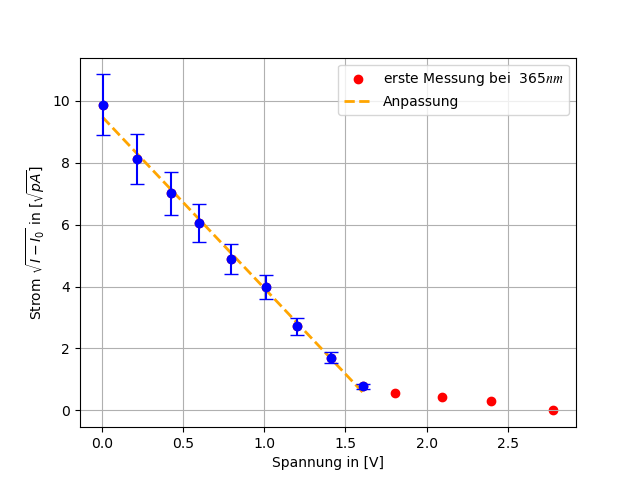
\includegraphics[width=.8\linewidth]{402_365nm_a.png}
  \caption{Auftragung der ersten Messung für $ \lambda =365nm$}
  \label{fig:wellenlaenge_365nm_a}
\end{figure}

\begin{figure}[h!]
  \centering
  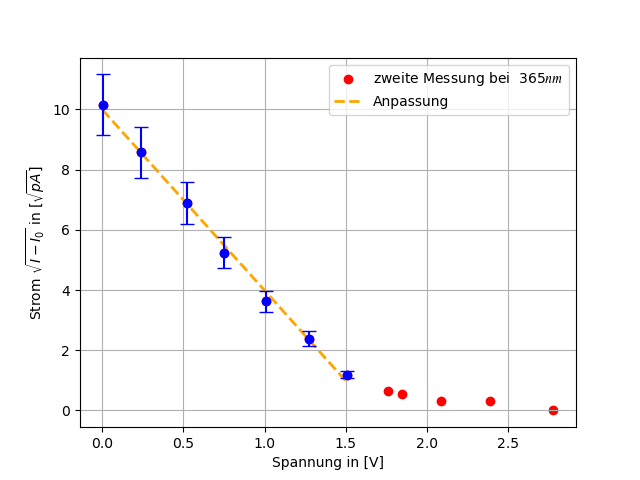
\includegraphics[width=.8\linewidth]{402_365nm_b.png}
  \caption{Auftragung der zweite Messung für $\lambda =365nm$}
  \label{fig:wellenlaenge_365nm_b}
\end{figure}

\begin{figure}[h!]
  \centering
  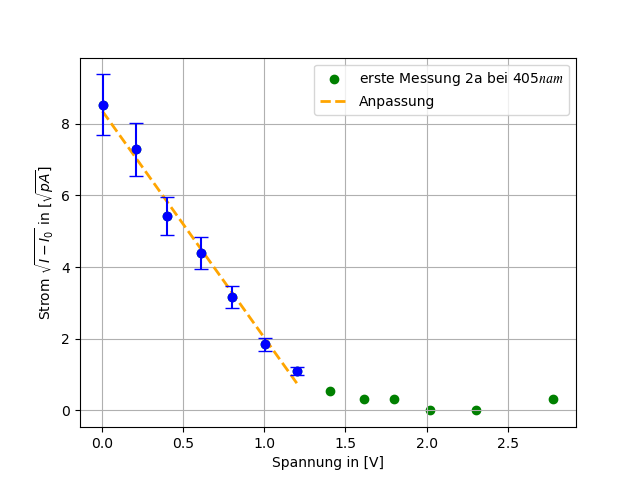
\includegraphics[width=.8\linewidth]{402_405nm_a.png}
  \caption{Auftragung der ersten Messung für $ \lambda =405nm$}
  \label{fig:wellenlaenge_405nm_a}
\end{figure}

\begin{figure}[h!]
  \centering
  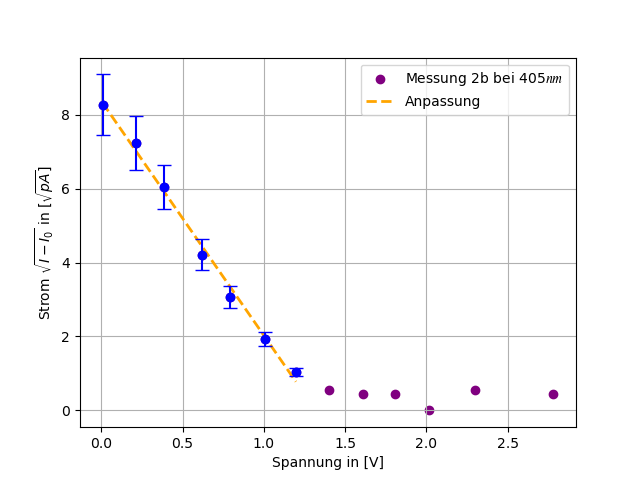
\includegraphics[width=.8\linewidth]{402_405nm_b.png}
  \caption{Auftragung der zweiten Messung für $\lambda =405nm$}
  \label{fig:wellenlaenge_405nm_b}
\end{figure}

\begin{figure}[h!]
  \centering
  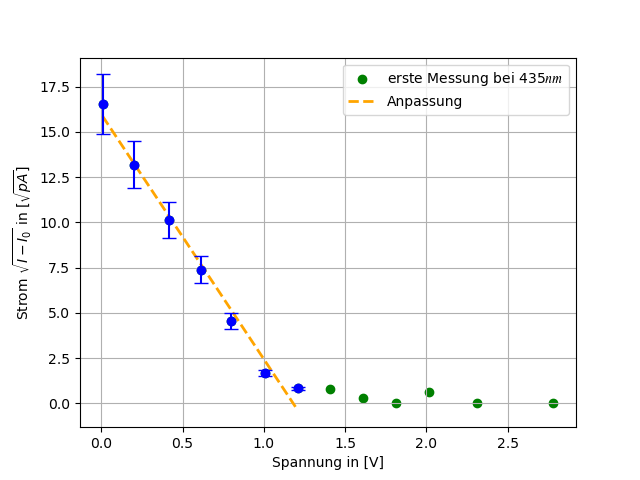
\includegraphics[width=.8\linewidth]{402_435nm_a.png}
  \caption{Auftragung der ersten Messung für $ \lambda =435nm$}
  \label{fig:wellenlaenge_435nm_a}
\end{figure}

\begin{figure}[h!]
  \centering
  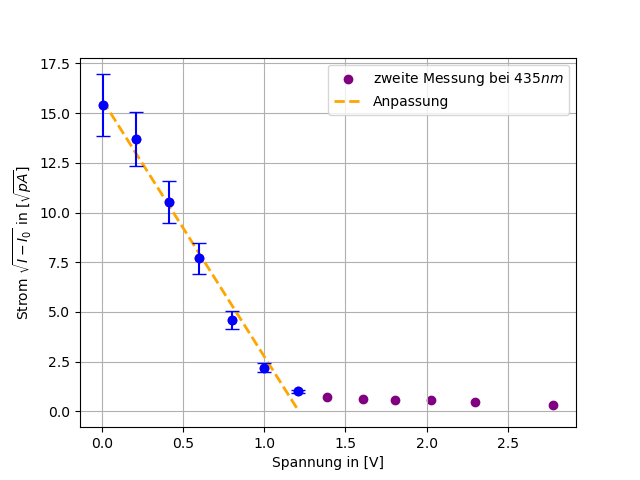
\includegraphics[width=.8\linewidth]{402_435nm_b.png}
  \caption{Auftragung der zweiten Messung für $\lambda =435nm$}
  \label{fig:wellenlaenge_435nm_b}
\end{figure}

\begin{figure}[h!]
  \centering
  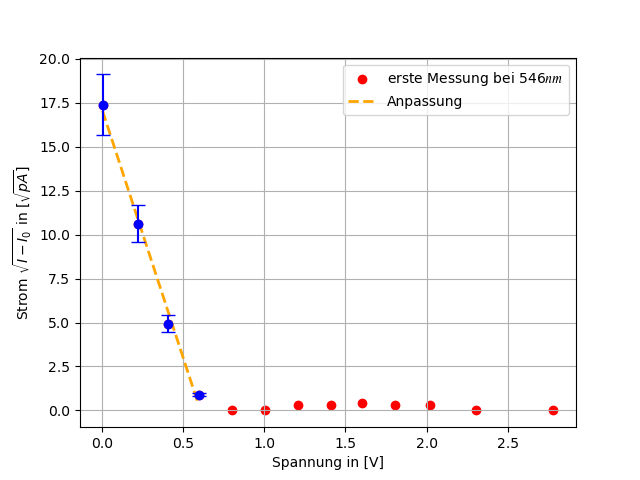
\includegraphics[width=.8\linewidth]{402_546nm_a.png}
  \caption{Auftragung der ersten Messung für $ \lambda =546nm$}
  \label{fig:wellenlaenge_546nm_a}
\end{figure}

\begin{figure}[h!]
  \centering
  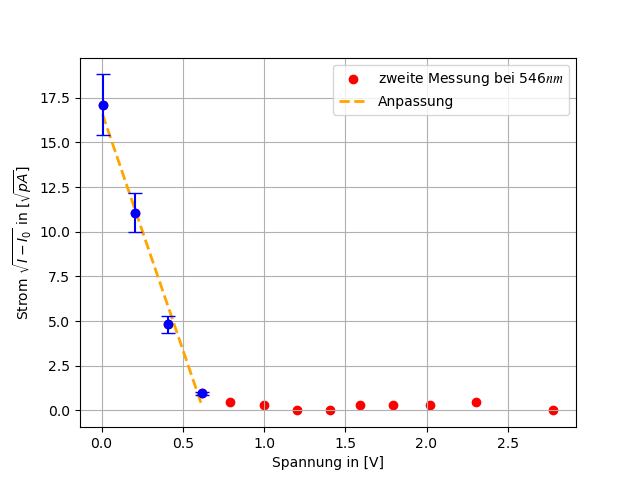
\includegraphics[width=.8\linewidth]{402_546nm_b.png}
  \caption{Auftragung der zweiten Messung für $\lambda =546nm$}
  \label{fig:wellenlaenge_546nm_b}
\end{figure}

\begin{figure}[h!]
  \centering
  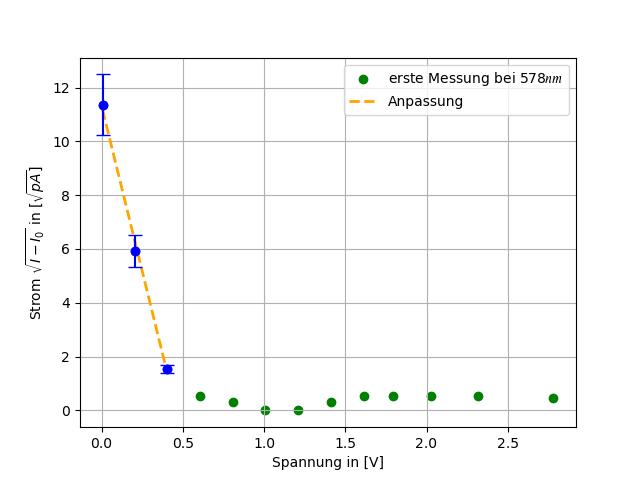
\includegraphics[width=.8\linewidth]{402_578nm_a.png}
  \caption{Auftragung der ersten Messung für $ \lambda =578nm$}
  \label{fig:wellenlaenge_578nm_a}
\end{figure}

\begin{figure}[h!]
  \centering
  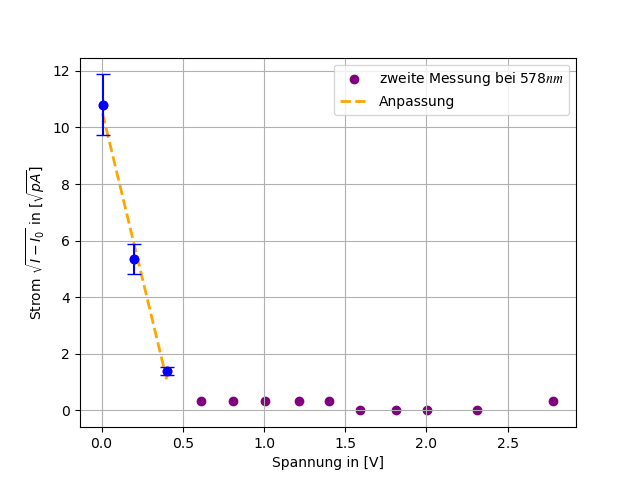
\includegraphics[width=.8\linewidth]{402_578nm_b.png}
  \caption{Auftragung der zweiten Messung für $\lambda =578nm$}
  \label{fig:wellenlaenge_578nm_b}
\end{figure}



\subsection{Balmer-Serie}
\begin{figure}[h!]
  \centering
  \begin{minipage}{0.49\textwidth}
    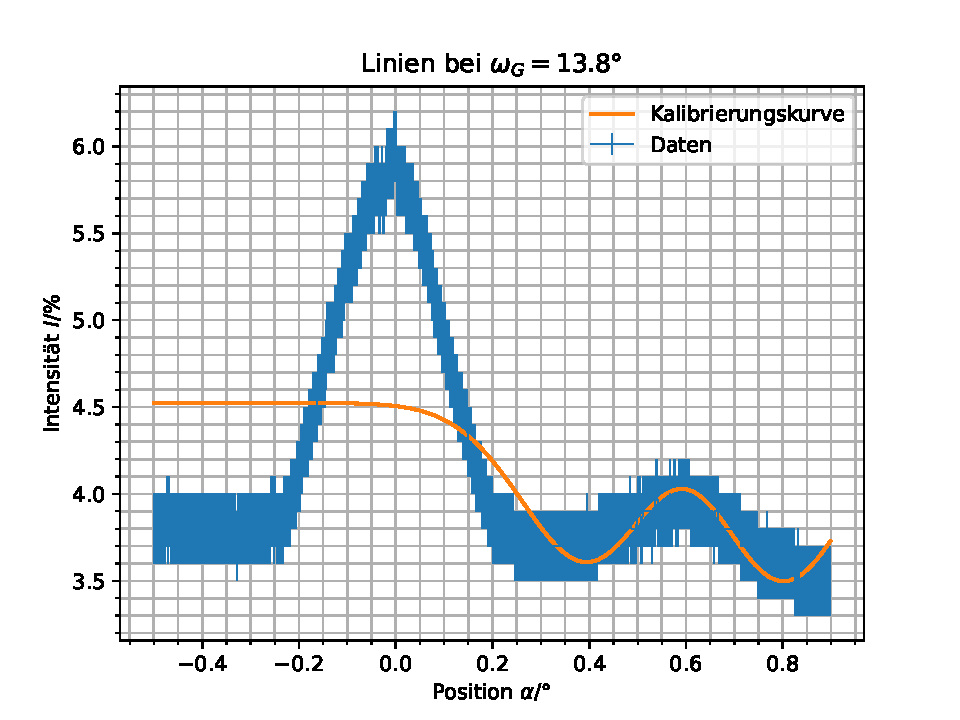
\includegraphics[width=\textwidth]{line13.8.pdf}
    \caption{CCD-Bild der Linie bei $\alpha=\ang{13.8}$.}
  \end{minipage}
  \hfill
  \begin{minipage}{0.49\textwidth}
    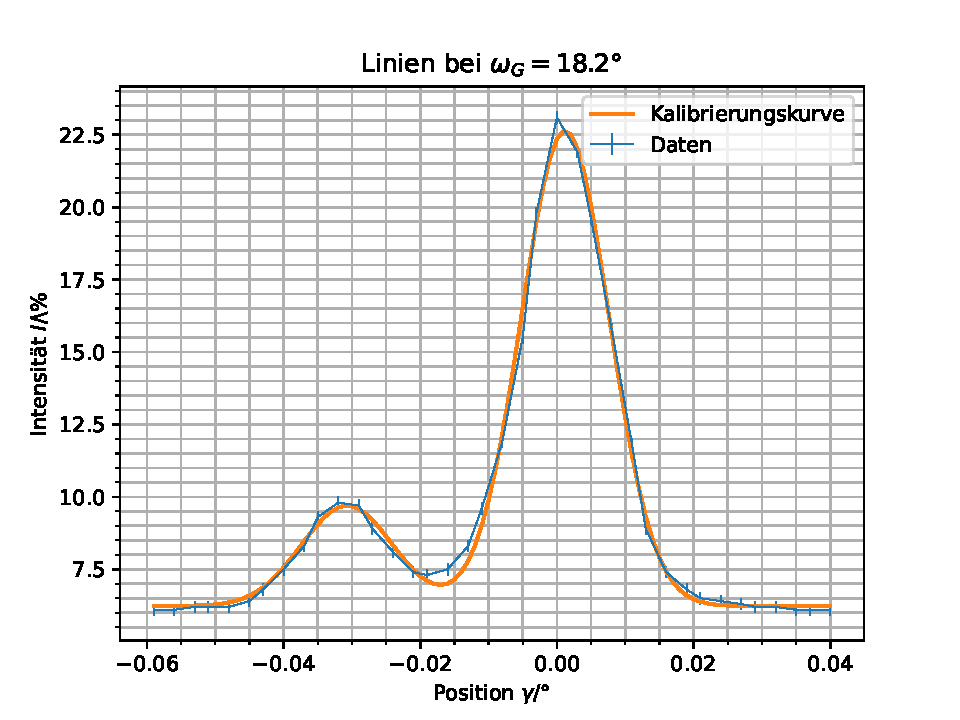
\includegraphics[width=\textwidth]{line18.2.pdf}
    \caption{CCD-Bild der Linie bei $\alpha=\ang{18.2}$ mit Fit.}
  \end{minipage}

  \begin{minipage}{0.49\textwidth}
    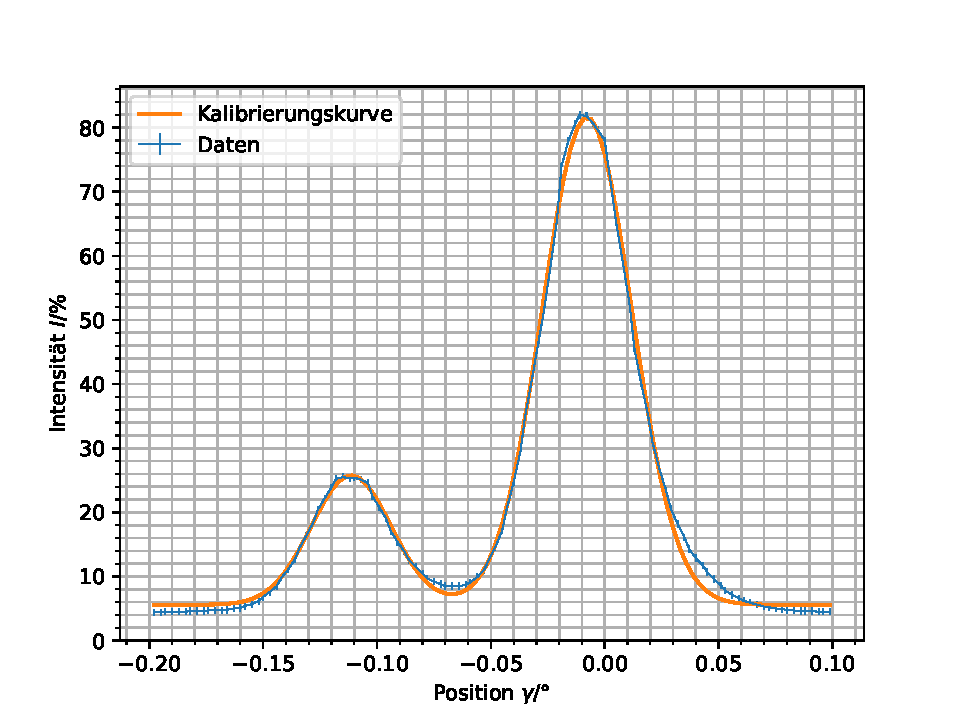
\includegraphics[width=\textwidth]{line37.0.pdf}
    \caption{CCD-Bild der Linie bei $\alpha=\ang{37.0}$ mit Fit.}
  \end{minipage}

  \label{fig:gauss-fit}
\end{figure}


\clearpage
\begin{thebibliography}{9}

\bibitem{Anleitung}
\textit{Physikalisches Praktikum Teil IV -- Versuchsbeschreibungen}, Universität Bonn, 10.10.2024

\bibitem{demtröder3}
\textit{Experimentalphysik 3 -- Atome, Moleküle, Festkörper}, 5. Auflage, Wolfgang Demtröder, 2016

\bibitem{leybold-balmer}
\textit{Balmer-Serie des Wasserstoff}, Leybold Didactic, Abruf 17.11.2024

\bibitem{elementarladung}
Wikipedia-Autoren, \textit{Elementarladung -- Wikipedia}, \url{https://de.wikipedia.org/wiki/Elementarladung}, Abruf 19.11.2024

\bibitem{rydberg}
\textit{The NIST Reference on Constants, Units, and Uncertainty}, NIST, https://physics.nist.gov/cgi-bin/cuu/Value?ryd, Abruf 19.11.2024

\bibitem{planck-h}
\textit{The NIST Reference on Constants, Units, and Uncertainty}, NIST, https://physics.nist.gov/cgi-bin/cuu/Value?h, Abruf 19.11.2024

\end{thebibliography}

\end{document}

